% Machine translated from the Danish original, ../danish/ad-problems-2023-trial.tex
% From the front page: CLRS refers to the course textbook, Introduction to Algorithms, 3rd edition.
\noindent\emph{This problem set has been machine translated from the Danish original.}
\medskip

\section*{Multiple-choice}\label{sec:mc}

\placeholder{Where to enter the multiple-choice answers, e.g.\ the multiple-choice module of the exam system.}

\multiplechoicestart


\question{MergeSort and comparisons}
Consider the following input to {\sc MergeSort}, implemented as in CLRS Section 2.3.
\begin{center}
\begin{tabular}{|c|c|c|c|c|c|c|c|}
\hline
42 & 33 & 36 & 43 & 11 & 38 & 22 & 66\\
\hline
\end{tabular}
\end{center}
How many times does {\sc MergeSort} compare the element 42 with another element of the input? (Comparisons with $\infty$ are not counted.)
\oneanswer
\optionsstart
\answer 3 comparisons
\answer 4 comparisons
\answer 5 comparisons \correct
\answer 6 comparisons
\answer 7 comparisons
\optionsend
\explanation{We can focus on the sorted lists that contain 42. One comparison is made to form the sorted list of 2 elements, 2 comparisons to form the sorted list of 4 elements, and another 2 comparisons to form the final sorted list. In total 5 comparisons.}
% 42 33 36 43 11 38 22 66
% 33 42 36 43 11 38 22 66  1 comparison
% 33 36 42 43 11 22 38 66  2 comparisons
% 11 22 33 36 38 42 43 66  2 comparisons


\question{MergeSort}
Suppose that {\sc MergeSort}$(A,p,r)$, implemented as in CLRS Section 2.3, is called on 21 elements (i.e., $r-p+1 = 21$).
How many calls to {\sc Merge-Sort} are made in total?
\oneanswer
\optionsstart
\answer 11
\answer 21
\answer 31
\answer 41 \correct
\answer 51
\optionsend
\explanation{The number of elements in each call of mergesort, grouped by recursion level, is: 21; 10, 11;5, 5, 5, 6; 2, 3, 2, 3, 2, 3, 3, 3; 1, 1, 1, 2, 1, 1, 1, 2, 1, 1, 1, 2, 1, 2, 1, 2; 1, 1, 1, 1, 1, 1, 1, 1, 1, 1. So the number of calls is $1+2+4+8+16+10 = 41$. Alternatively, one can observe that the total number of nodes in a binary tree with 21 leaves in which every internal node has two children is always $2\cdot 21 - 1 = 41$.}


\question{Shortest-paths tree}
Consider a single-source shortest-paths problem on a graph $G=(V,E)$
with weight function $w: E\rightarrow \mathbb{R}$ and source vertex $s$.
Which of the following properties does a shortest-paths tree $G'=(V',E')$ always have?
\multipleanswers
\optionsstart
\answer In $G'$ all vertices in $V$ are reachable from $s$.
\answer The vertex $s$ has only outgoing edges in $G'$. \correct
\answer $G'$ has $|V'|-1$ edges. \correct
\answer If all weights are distinct, $G'$ contains the $|E'|$ edges of $G$ that have the lowest weights.
\answer $G'$ contains the edge of $G$ that has the lowest weight.
\optionsend
\explanation{$G'$ only connects $s$ with the vertices in $V$ to which there is a path in $G$.
There are only outgoing edges from $s$ because the tree has no cycles.
$G'$ is a tree, and therefore the number of edges equals the number of vertices minus 1.
A low weight is no guarantee of being on a shortest path from $s$ --- for example, some edges may not be reachable from~$s$.
}


\question{Shortest paths}
Consider the single-source shortest-paths problem with source vertex {\bf a} on the following graph:
\begin{center}
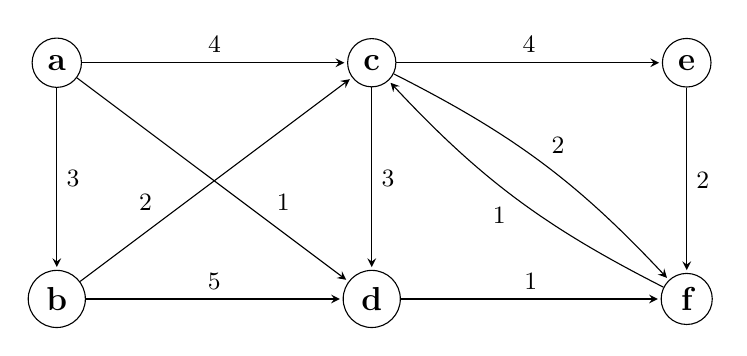
\begin{tikzpicture}[->,>=stealth,shorten >=1pt,auto,
    main node/.style={circle,draw,font=\large\bfseries}]
\node[main node] (a) at (2,1.5) {a};
\node[main node] (b) at (2,-1.5) {b};
\node[main node] (c) at (6,1.5) {c};
\node[main node] (d) at (6,-1.5) {d};
\node[main node] (e) at (10,1.5) {e};
\node[main node] (f) at (10,-1.5) {f};

\path[every node/.style={font=\small}]
(a) edge node {3} (b)
edge node {4} (c)
edge node[pos=0.7] {1} (d)
(b) edge node[pos=0.3] {2} (c)
edge node {5} (d)
(c) edge node {3} (d)
edge [bend left=10] node {2} (f)
edge node {4} (e)
(d) edge node {1} (f)
(e) edge node {2} (f)
(f) edge [bend left=10] node {1} (c);
\end{tikzpicture}
\end{center}
Which edges are in the shortest-paths tree?
\multipleanswers
\optionsstart
\answer (a,b) \correct
\answer (a,c)
\answer (a,d) \correct
\answer (b,c)
\answer (b,d)
\answer (c,d)
\answer (c,e) \correct
\answer (c,f)
\answer (d,f) \correct
\answer (e,f)
\answer (f,c) \correct
\optionsend
\explanation{Since there are only positive weights, the edges of the tree can be found by running Dijkstra's algorithm, which gives the output indicated (which is unique in this case).}


\question{Minimum spanning tree}
Consider the minimum spanning tree problem on this graph:
\begin{center}
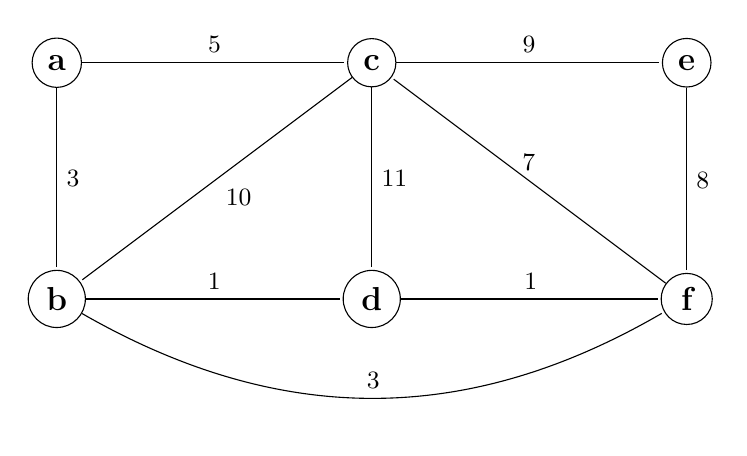
\begin{tikzpicture}[-,>=stealth,shorten >=1pt,auto,
    main node/.style={circle,draw,font=\large\bfseries}]
\node[main node] (a) at (2,1.5) {a};
\node[main node] (b) at (2,-1.5) {b};
\node[main node] (c) at (6,1.5) {c};
\node[main node] (d) at (6,-1.5) {d};
\node[main node] (e) at (10,1.5) {e};
\node[main node] (f) at (10,-1.5) {f};

\path[every node/.style={font=\small}]
(a) edge node {3} (b)
edge node {5} (c)
(b) edge node {1} (d)
edge[bend right=30] node {3} (f)
(c) edge node {11} (d)
edge node {9} (e)
edge node {10} (b)
(d) edge node {1} (f)
(e) edge node {8} (f)
(f) edge node[above] {7} (c);
\end{tikzpicture}
\end{center}
Which edges are in the minimum spanning tree?
\multipleanswers
\optionsstart
\answer \{a,b\} \correct
\answer \{a,c\} \correct
\answer \{b,c\}
\answer \{b,d\} \correct
\answer \{b,f\}
\answer \{c,d\}
\answer \{c,e\}
\answer \{c,f\}
\answer \{d,f\} \correct
\answer \{e,f\} \correct
\optionsend
\explanation{A minimum spanning tree can be found by running, e.g., Kruskal's or Prim's algorithm, which gives the output indicated (which is unique in this case).}



\question{Red-black search trees}
Consider this red-black binary search tree, where the leaves are omitted from the drawing:
%
\begin{center}
\begin{tikzpicture}[-,>=stealth,level/.style={sibling distance = 5cm/#1,
    level distance = 1cm}]
  \node [black] {10}
      child{ node [red] {3}
              child{ node [black] {1}
              }
              child{ node [black] {8}
              }
      }
      child{ node [black] {15}
              child{ node [red] {12}
              }
              child{ node [red] {17}
              }
          }
  ;
  \end{tikzpicture}
\end{center}

\medskip

Suppose we use the insertion algorithm {\sc RB-Insert} from CLRS Chapter 13 to insert the key~9. What happens to the tree?
\oneanswer
\optionsstart
\answer 9 is inserted as the right child of node 8 and colored red. \correct
\answer 9 is inserted as the right child of node 8 and colored black.
\answer 9 is inserted as the left child of node 12 and colored red.
\answer 9 is inserted as the left child of node 12 and colored black.
\answer None of the above.
\optionsend
\explanation{ {\sc RB-Insert} finds the right place in the tree for the key 9, as the right child of node 8. The node is colored red and then {\sc RB-Insert-Fixup} is called, but it terminates without changing anything because the parent node 8 is black.
}


\question{Running time of red-black search trees}
Consider a red-black binary search tree $T$, as described in CLRS Chapter 13,
on which $n_1$ {\sc Insert} operations, $n_2$ {\sc Delete} operations, and $n_3$ {\sc Search} operations (the latter are also called ``access'' operations) are performed.
The total number of operations is $N=n_1+n_2+n_3$.
Which of the following statements are always true?
\multipleanswers
\optionsstart
\answer The total time for the operations is $\Omega(N)$. \correct
\answer The total time for the operations is $O(N \lg N)$. \correct
\answer The total time for the operations is $O(n_3 + (n_1 + n_2) \lg N)$.
\answer The depth of $T$ is at most $2\lg(n_1 + 1)$. \correct
\answer All leaves of $T$ are at depth at least $\lfloor \lg(n_3 + 1)\rfloor$.
\answer All black nodes of $T$ are at an even distance from the root.
\optionsend
\explanation{ Each operation takes at least constant time, so the total time is $\Omega(N)$. The number of nodes $n$ in the tree is at any time at most $n_1 \leq N$. So each operation takes at most $O(\lg N)$ time, and the total time is $O(N \lg N)$. In the worst case the search operations take time $\Omega(\lg n_1)$, i.e., time $\Omega(n_3\lg n_1)$ in total, so the time cannot be bounded by $O(n_3 + (n_1 + n_2) \lg N)$. A red-black binary search tree can have leaves at depth 2 regardless of the value of $n_3$, so in general the leaves are not necessarily at depth at least $\lfloor \lg(n_3 + 1)\rfloor$. Black nodes can occur at all levels.
}



\question{Amortized analysis}
In this problem we consider the potential function used to analyze dynamic tables in CLRS Section 17.4.1.
Let $\Phi_i$ denote the value of the potential function after $i$ {\sc Table-Insert} operations, without any {\sc Table-Delete} operations.
Which properties does $\Phi_i$ have?
\multipleanswers
\optionsstart
\answer $\Phi_i = \Omega(1)$.\correct
\answer $\Phi_i = O(1)$.
\answer $\Phi_i = \Omega(i)$.
\answer $\Phi_i = O(i)$.\correct
\answer $\Phi_{i} \geq \Phi_{i-1}$.
\answer $\Phi_{i} \geq 0$. \correct
\optionsend
\explanation{ $\Phi_i = 2\cdot num_i - size_i$, where $num_i = i$ and $size_i \geq 1$ is the current capacity. We always have $\Phi_i \leq i$, so $\Phi_i=O(i)$, but right after a table expansion we have $\Phi_i \leq 2$, i.e., it does not hold that $\Phi_i = \Omega(i)$. Right after a table expansion we have $\Phi_{i} < \Phi_{i-1}$. The potential function is defined so that it is non-negative, and it is positive from the first step onward.
}


\question{Divide and conquer}
Which of these recurrences have the solution
$T(n) = \Theta(n^2)$? Assume that $T(n)=1$ for $n\leq 1$.
\multipleanswers
\optionsstart
\answer $T(n) = 4 T(\lfloor n/2\rfloor ) + n \lg n$. \correct
\answer $T(n) = 4 T(\lfloor n/2\rfloor ) + n^2$.
\answer $T(n) = 2 T(\lfloor n/4\rfloor ) + n^2$. \correct
\answer $T(n) = 9 T(\lfloor n/3\rfloor ) + n^3$.
\answer $T(n) = T(n-1) + n^2$. % Cannot be solved with the master theorem in CLRS
\answer $T(n) = T(n-1) + n$. \correct % Cannot be solved with the master theorem in CLRS
\optionsend
\explanation{ The first four recurrences can be solved using the master theorem, where numbers 1 and 3 fall in cases 1 and 3, respectively, which give $T(n) = \Theta(n^2)$.
The last recurrences can be solved with the substitution method.
In recurrence 5 there are $n$ terms, half of which have size at least $(n/2)^2 = n^2/4$, so $T(n)=\Omega(n^3)$.
In recurrence 6 there are $n$ terms of size at most~$n$, half of which have size at least $n/2$, so $T(n)=\Theta(n^2)$.
}



\multiplechoiceend



\newpage


\section*{Written problems}\label{sec:written}

% Machine translated from the Danish original, ../danish/skriftlige.tex
{\bf Written problems:} \placeholder{How the answers are submitted, e.g.\ the file format and exam system, and whether drawings made on a tablet may be inserted.}
\begin{itemize}
    \item Use \emph{one page for each subquestion, in the same order as in the problem set.}
    \item The number/letter of the subquestion (e.g.\ 19 or 20.a) must be stated.
\end{itemize}



\section{Huffman tree (4\%)}

We consider the algorithm for constructing Huffman codes in CLRS Section 16.3.

\subquestion{a)}{Draw the Huffman tree that the algorithm computes for the alphabet $C =\{a, b, c, d, e\}$ with frequencies $f_a=5$, $f_b=8$, $f_c=3$, $f_d=7$, $f_e=1$.
It is not necessary to give labels (0 and 1) on the edges, but state the frequencies in leaves as well as internal nodes (see the example in CLRS Figure~16.4).}

\explanation{The algorithm computes this tree (drawn without 0-1 labels on the edges):\medskip
\begin{center}
    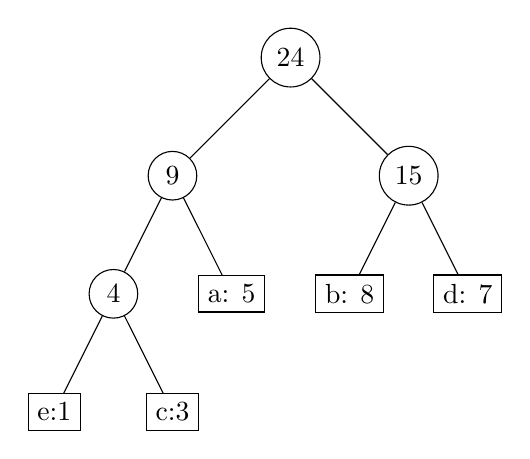
\begin{tikzpicture}[level distance=1.5cm,  level 1/.style={sibling distance=3cm},  level 2/.style={sibling distance=1.5cm}]
        \node [circle, draw] {24}
          child {node [circle, draw] {9}
            child {node [circle, draw] {4}
              child {node [rectangle, draw] {e:1}}
              child {node [rectangle, draw] {c:3}}
            }
            child {node [rectangle, draw] {a: 5}}
          }
          child {node [circle, draw] {15}
            child {node [rectangle, draw] {b: 8}}
            child {node [rectangle, draw] {d: 7}}
          };
      \end{tikzpicture}
\end{center}
}



\section{Dynamic programming (10\%)}

We consider the following variant of the \emph{rod cutting} problem from CLRS Section 15.3.
The input is an integer $n$ and a vector $p$, where $p_i$ is the revenue for a rod of length $i$.
As in rod cutting, a rod of length $n$ must be cut into shorter rods, all of integer length, so that the total revenue is maximized.
Unlike the original rod cutting problem, however, there is a cost of 1 for each cut, which must be subtracted from the revenue.

\medskip

{\bf Example.} Suppose we have a rod of length $n=5$, where $p = (p_1,p_2,p_3,p_4,p_5) = (1,3,5,6,6)$. If we cut the rod into two pieces of sizes 2 and 3, respectively, the revenue is $p_2 + p_3 - 1 = 7$, where we subtract $1$ because there is one cut. If we instead cut it into 5 pieces of size 1, the revenue would be $5\,p_1 - 4 = 1$.


\subquestion{a)}{Write a recurrence for the revenue $r_n$ for a rod of length $n$.}

\explanation{We have $r_0 = 0$, and by the same argument as for standard rod cutting, $r_n = \max\bigl(p_n, \max_{1\leq i \leq n-1} (p_i + r_{n-i} - 1)\bigr)$ for $n\geq 1$, where we subtract 1 because of the cost of the cut between the first piece of length $i$ and the rest (if the rod is sold whole for $p_n$, no cut is made).}

\subquestion{b)}{Analyze the running time of an algorithm that uses the recurrence and dynamic programming to compute the revenue for a rod of length $n$. The analysis must give an upper bound on the running time as a function of $n$ in big-$O$ notation that is as precise as possible.}

\explanation{The analysis for rod cutting can be reused, since the recurrence has the same structure. The change only affects the values, and the time for each step increases by at most a constant factor. Hence the running time is $O(n^2)$.}



\section{Proofs by induction (6\%)}

In this problem we consider $n$-gons such as these examples ($n=4$ and $n=6$):
\begin{center}
\begin{tikzpicture}
  \draw (0,0) -- (2,0) -- (2,2) -- (0,2) -- (0,0);
\end{tikzpicture}
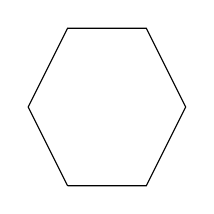
\begin{tikzpicture}
  \draw (0,0) -- (1,0) -- (1.5,1) -- (1,2) -- (0,2) -- (-0.5,1) -- (0,0);
\end{tikzpicture}
\end{center}
%
We are interested in the number of \emph{diagonals}, i.e., line segments that connect two corners of the $n$-gon and lie entirely inside the figure. A 3-gon has no diagonals, since all corners are neighbors, while for $n=4$ and $n=6$ we have 2 and 9 diagonals, respectively.
\begin{center}
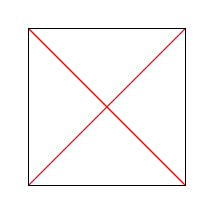
\begin{tikzpicture}
  \draw[red] (0,0) -- (2,2);
  \draw[red] (0,2) -- (2,0);
  \draw (0,0) -- (2,0) -- (2,2) -- (0,2) -- (0,0);
\end{tikzpicture}
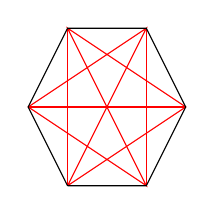
\begin{tikzpicture}
  \draw[red] (0,0) -- (0,2);
  \draw[red] (1,0) -- (1,2);
  \draw[red] (-0.5,1) -- (1.5,1);
  \draw[red] (0,0) -- (1.5,1) -- (0,2) -- (1,0) -- (-0.5,1) -- (1,2) -- (0,0) -- (1,2) -- (-0.5,1) -- (1,0) -- (0,2) -- (1.5,1);
  \draw (0,0) -- (1,0) -- (1.5,1) -- (1,2) -- (0,2) -- (-0.5,1) -- (0,0.0);
\end{tikzpicture}
\end{center}
A diagonal divides an $n$-gon into an $n_1$-gon and an $n_2$-gon that share an edge, where $n_1 + n_2 = n + 2$. For example, a diagonal of the 4-gon divides it into two 3-gons.

\subquestion{a)}{Prove by induction that the number of diagonals $d_n$ in an $n$-gon equals $n(n-3)/2$ for $n\geq 3$.
Emphasis is placed on the argument being clear and concise.
}

\explanation{For $n=3$ we have $d_n = 0 = 3(3-3)/2$, which establishes the base case. Now assume that $n>3$, that the statement holds for $n'$-gons with $n'<n$, and consider an $n$-gon.
Take three adjacent corners $v_1, v_2, v_3$, i.e., such that $v_1$ and $v_3$ are connected to $v_2$.
From $v_2$ we can draw diagonals to each of the other $n-3$ corners, and
in addition we can draw a diagonal between $v_1$ and $v_3$.
The remaining diagonals lie in the $(n-1)$-gon obtained by leaving out $v_2$ (and connecting $v_1$ and $v_3$ directly).
By the induction hypothesis there are $d_{n-1}=(n-1)(n-4)/2$ diagonals in this part, i.e.,
%
\[ d_n = n-3 + 1 + d_{n-1} = n-2 + (n-1)(n-4)/2 = n(n-3)/2 \enspace . \]
}



\section{Correctness and running time (10\%)}\label{sec:last}

In this problem we use matrix and vector notation; see, e.g., CLRS Appendix D.1.
The Fibonacci numbers $F_0, F_1, F_2,\dots$ are defined by $F_0 = 0$, $F_1 = 1$, and $F_{n} = F_{n-1} + F_{n-2}$ for $n>1$.
Now consider the matrix $A$ and column vectors of the form $x = (x_1, x_2)^T$.

\[
 A =   \begin{pmatrix}
        0 & 1 \\
        1 & 1
    \end{pmatrix}
\qquad x =
\begin{pmatrix}
    x_1\\
    x_2
\end{pmatrix}
\]

\subquestion{a)}{Argue that for $x = (F_{n-2}, F_{n-1})^T$ the matrix-vector product satisfies the equality $A x = (F_{n-1}, F_{n})^T$ for $n>1$.}

\explanation{By the definition of matrix-vector products we have:
\[
 \begin{pmatrix}
        0 & 1 \\
        1 & 1
    \end{pmatrix}
\begin{pmatrix}
    F_{n-2}\\
    F_{n-1}
\end{pmatrix}
=
\begin{pmatrix}
    F_{n-1}\\
    F_{n-2} + F_{n-1}
\end{pmatrix}
=
\begin{pmatrix}
    F_{n-1}\\
    F_{n}
\end{pmatrix},
\]
where the last equality uses the definition of $F_n$.
}

\subquestion{b)}{Prove that for $x = (0,1)^T$ the equality $A^{n-1} x = (F_{n-1}, F_{n})^T$ holds for $n\geq 1$.}

\explanation{
Proof by induction on $n$.
The base case $n=1$ holds since $A^{n-1} x = x = (F_0, F_1)^T$.
Assume as the induction hypothesis that $A^{i-1} x = (F_{i-1}, F_{i})^T$ for $1\leq i < n$.
Then we have%
\[
    A^{n-1} x = A(A^{n-2} x) = A (F_{n-2}, F_{n-1})^T = (F_{n-1}, F_{n})^T,
\]
where the second equality uses the induction hypothesis and the third equality uses part a).
}

\subquestion{c)}{Argue that $A^{n-1}$, and hence also $A^{n-1} x$, can be computed in time $O(\lg n)$, assuming that arithmetic operations take constant time.}

\explanation{
    We have the following recurrence:
    \begin{equation*}
        A^n = \begin{cases}
        I & \text{ if } n=0\\
        (A^{n/2})^2 &\text{ if } n > 0 \text{ is even}\\
        A (A^{(n-1)/2})^2 &\text{ if } n \text{ is odd}
        \end{cases}
    \end{equation*}
Since $A^n$ has constant size, this means that $A^n$ can be computed in constant time from either $A^{n/2}$ or $A^{(n-1)/2}$.
This gives recursion depth at most $\lg(n)$, and hence time $O(\lg n)$.
}



\label{page:last}
